%%%%%%%%%%%%%%%%%%%%%%%%%%%%%%%%%%%%%%%%%%%%%%%%%%%%%%%%%%%%%%%%%%%%%%%%%%%%%%%%
%2345678901234567890123456789012345678901234567890123456789012345678901234567890
%        1         2         3         4         5         6         7         8

\documentclass[letterpaper, 10 pt, conference]{ieeeconf}  % Comment this line out if you need a4paper

%\documentclass[a4paper, 10pt, conference]{ieeeconf}      % Use this line for a4 paper

\IEEEoverridecommandlockouts                              % This command is only needed if
                                                          % you want to use the \thanks command

\overrideIEEEmargins                                      % Needed to meet printer requirements.

% See the \addtolength command later in the file to balance the column lengths
% on the last page of the document

% The following packages can be found on http:\\www.ctan.org
%\usepackage{graphics} % for pdf, bitmapped graphics files
%\usepackage{epsfig} % for postscript graphics files
%\usepackage{mathptmx} % assumes new font selection scheme installed
%\usepackage{times} % assumes new font selection scheme installed
%\usepackage{amsmath} % assumes amsmath package installed
%\usepackage{amssymb}  % assumes amsmath package installed
\usepackage{graphicx}
\usepackage[export]{adjustbox}
\graphicspath{ {images/} }

\usepackage{tabularx}
\usepackage{xcolor}
\newcommand\ytl[2]{
\parbox[b]{8em}{\hfill{\color{cyan}\bfseries\sffamily #1}~$\cdots\cdots$~}\makebox[0pt][c]{$\bullet$}\vrule\quad \parbox[c]{4.5cm}{\vspace{7pt}\color{red!40!black!80}\raggedright\sffamily #2.\\[7pt]}\\[-3pt]}

\title{\LARGE \bf
Robot Manipulator Proposal
}


\author{ Thibaut Marmey and Louis Gatin, Ludovic Bouan, Ni-Ching Lin, Hani Hassan  % <-this % stops a space
\thanks{*This work was supported by the Robotics Master Program in National Chiao Tung University, Taiwan}% <-this % stops a space
}


\begin{document}


\maketitle
\thispagestyle{empty}
\pagestyle{empty}


\section{INTRODUCTION \& MOTIVATION}

Amazon is able to quickly package and ship millions of items to customers from a network of fulfillment centers all over the globe.
This wouldn't be possible without leveraging cutting-edge advances in technology. Amazon's automated warehouses are successful at removing much of the walking and searching for items within a warehouse.

However, commercially viable automated picking and stowing in unstructured environments still remains a difficult challenge.
In order to spur the advancement of these fundamental technologies, Amazon Robotics organizes the Amazon Robotics Challenge (ARC)~\cite{APC}.
In recent years, ARC has become famous, and many scholars dedicated themselves to this competition and hope to show off their talents. The goal of the challenge was to design an autonomous robot to pick items from a warehouse shelf. Amazon provided a set of objects from 39 categories, representing a large variety of challenging properties, including heavy objects, flat objects, and non-solid objects with many holes (see figure~\ref{figure:items}).

Actually, picking problems arise in a wide range of applications, from industrial automation to personal service robots. Kinds of different grippers have different utility and signification. Combining adaptive grippers and vacuum cups could create the best grip for ARC. The advantage of the adaptive gripper is its ability to envelope the objects according to its geometric shapes. While the vacuum cups could cover the weaknesses of a gripper such as gripping flat objects or other difficult shapes.

In this project, we would like to present our innovative gripper, which have two stems (Figure~\ref{figure:gripper}) to grab object and one suction cup. Those stems can stay parallel or they have the possibility to close themselves like fingers. Those different moves can permit to be more efficient for picking objects. The positions of the stems are controlled with two motors so mathematical analysis will be necessary. The suction cup can be place on one stem or we can create an other arm for this purpose only. We need to add pressure sensors for picking feedbacks. We think about sensors with many pressure cells because we could be able to know the position of the contact between the object and the stems and adjust it. An embedded controller will control everything on the manipulator and communicate with robot operation system (ROS). ROS is well-designed as an manipulator control system and robot communication system. Using ROS message we could use easy command to control the gripper and with the manipulator.

Our motivation stems from our will to be part of a very challenging competition and think about it as a global project in a real environment. This project deals with a lot of different topics and our combined experience is necessary to complete the tasks. Our team members have different electrical, control, and mechanical backgrounds, which is a great strength for us to exploit. With this project, we will understand how ROS works and how it interacts with all parts of the robot.

\begin{figure}[t]
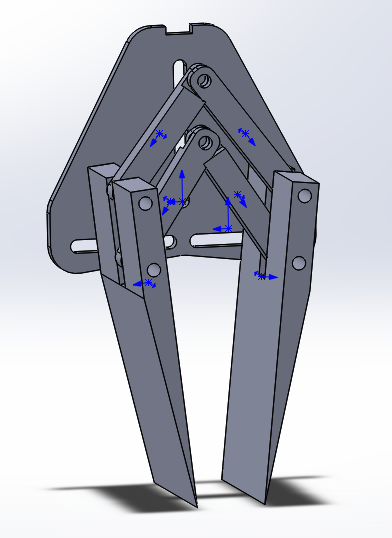
\includegraphics[width=0.95\columnwidth]{gripper}
\centering
\caption{Gripper (without vacuum cup)}
\label{figure:gripper}
\end{figure}

\section{SYSTEM ARCHITECTURE \& EQUIPMENTS}


\subsection{SYSTEM ARCHITECTURE}


Our system aims to provide suction, parallel, and multi-joint gripping. These are the major gripping components. They are controlled via an air and an electrical connection. An Arduino receives instructions from the robot and acts upon the control in accordance to the instructions. Figure ~\ref{figure:system} outlines the global structure of the system. Figure ~\ref{figure:cinematic} is a link diagram showing the proposed mechanical design.

The development of our manipulator is centered on 4 poles: mechanical, software, electrical/pneumatic, and gripping. The four majors tasks to be taken on are:
\begin{enumerate}
  \item Create the mechanical design of the gripper. The design must be reliable, 3D-printable, have multiple joints, suction cups, and good gripping capability, and a minimum space requirement.
  \item Programming of the control unit. The Arduino must be programmed to control the electric motors and valves according to ROS messages received from the robot.
  \item Design and build the electrical and pneumatic circuits.
  \item Design and build the figertip grippers.
\end{enumerate}


\begin{figure}[h]
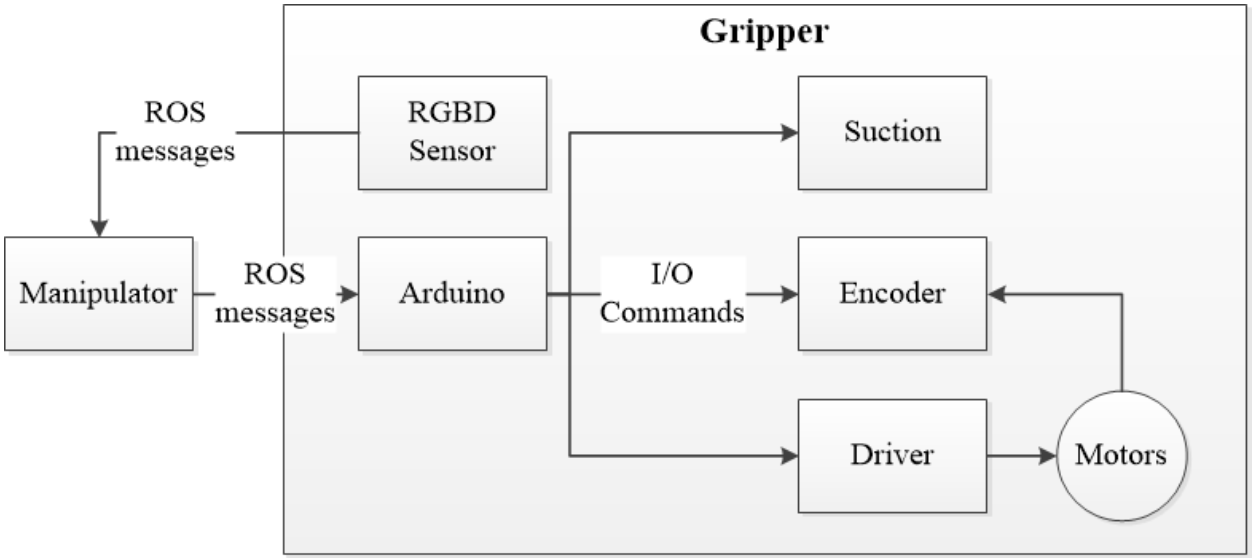
\includegraphics[width=0.7\columnwidth]{system}
\centering
\caption{System overview}
 \label{figure:system}
\end{figure}

\begin{figure}[h]
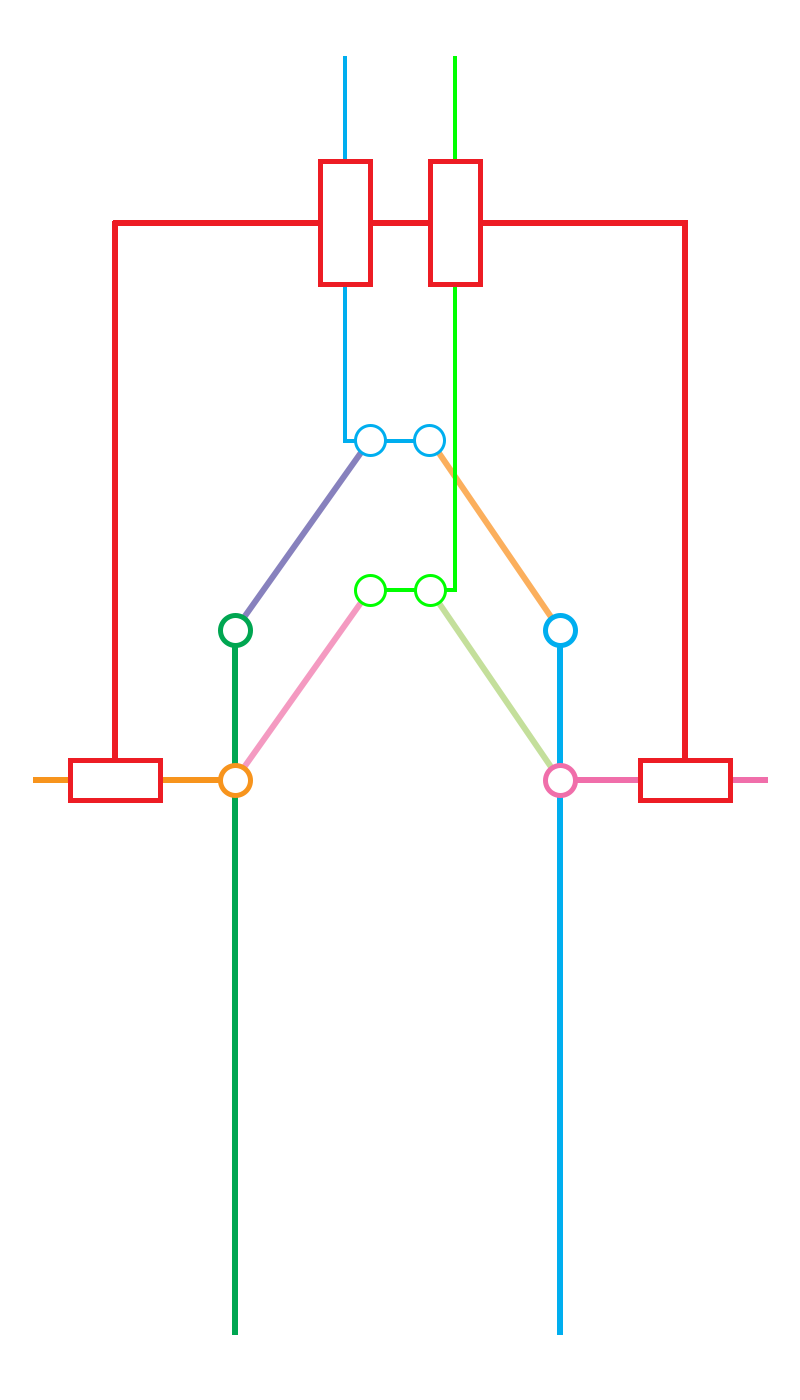
\includegraphics[width=0.7\columnwidth]{cinematic}
\centering
\caption{Cinematic link diagram}
 \label{figure:cinematic}
\end{figure}

\begin{figure}[t]
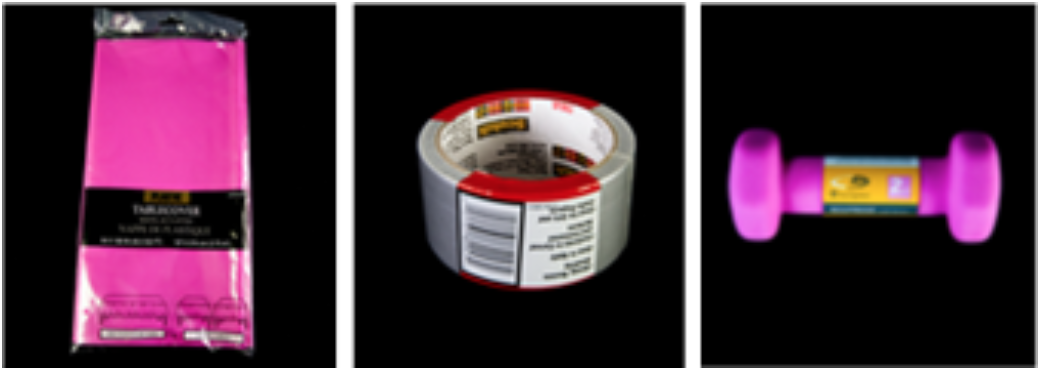
\includegraphics[width=0.95\columnwidth]{items}
\centering
\caption{Items from APC 2017}
\label{figure:items}
\end{figure}

\newpage
\subsection{EQUIPMENTS}

Table ~\ref{table:equipment} lists the equipment needed for our project.

\begin{table}[h]
\centering
\caption{Equipment Needed}
\label{my-label}
% \begin{tabular}{lll}
\begin{tabularx}{\linewidth}{|m{0.2\linewidth}|l|X|}
  \hline
\textbf{Name}    & \textbf{Quantiy} & \textbf{Purpose}                                                                           \\ \hline
3D-printer       & 1         & Print the various components of our manipulator                                                   \\ \hline
Air pump         & 1         & Create a source of high-pressure air for the vacuum generator                                     \\ \hline
Arduino nano     & 1         & Control unit for the manipulator                                                                  \\ \hline
Electric motor   & 2 or 3    & Actuate the moving parts of the manipulator                                                       \\ \hline
Vacuum cups      & 1         & Provide better grip and grasping capabilities                                                     \\ \hline
Vacuum generator & 1         & Create vacuum for the suction cups                                                                \\ \hline
Control Valve    & 1         & Control the air supply to the vacuum cups                                                         \\ \hline
RGB Sensor       & 1         & Relay data to the robot's main computer                                                           \\ \hline
Power Supply     & 1         & For powering and testing onboard electronics                                                      \\ \hline
Various          & -         & Cabling, wiring, connectors, and other various small mechanical and electrical parts for assembly \\ \hline
\end{tabularx}
\label{table:equipment}
\end{table}

\section{SPECIFIC AIMS}

As the task for designig a robot which its main task is going to pick, place and handle different Items with different shapes, materials and surfaces, this chalanges inspired me and my teammates with an idea for producing a stable and safe mechanical design for a multi function gripper that can handle items with different shapes dynamically, easily, precisly and in less time, As well as to add a sensing and intelegent systems to assure a the complition of the function needed successfuly. 


\section{APPROACH}

As some of our chalanges is to maintain handling items easily and precisly in addition to adding sensable and intellegent feedback systems, I got an idea of implenting a design for a system ispired by the the distal phalanges of human's hand, which is going to be modeled as two small air bags that could change its internal pressure depend on the the item needed to be handled. 
The idea came as the gripper is gonna have an air flow system as our team is already going to add a suction cup to the gripper, so the finger will be adjust the internal pressure of the bags automatically to assure a high contact area to hold the item as well as the bags will be made from rubbery material that will produce high frictional grip, we are seeking to add an feed back system which will mainly consist of a pressure sensor that will detect the increase of internal pressure, and intellengtly will adjust the pressure suitable for each item.

\section{SCHEDULE AND TEAM COLLABORATION}

Table ~\ref{table:personal_timeline} shows the timeline for achieving my specific aims. Figure ~\ref{figure:gantt} shows the entire team's schedule.

\begin{table}[h]
\caption{Personal Timeline of project}
%\centering
%\begin{minipage}[t]{.7\linewidth}
\color{gray}
%\rule{\linewidth}{1pt}
\ytl{Nov 07}{Review of proposal and definition of project goals with team members}
\ytl{Nov 14}{Research dimensions of overall gripper and technologies to use}
\ytl{Nov 21}{Collaboration with electrical design to choose the actuators, first design release}
\ytl{Nov 28}{Start the mechanical analysis based on the model}
\ytl{Dec 05}{Finish the mechanical analysis and collaboration with software design}
\ytl{Dec 12}{Optimize the pieces design to be 3D-printed, print them}
\ytl{Dec 19}{Integration testing and assembly in collaboartion with software and electrical design}
\ytl{Dec 26}{Write conclusions and paper}
\ytl{Jan 02}{Prepare presentation}
%\bigskip
\label{table:personal_timeline}
%\rule{\linewidth}{1pt}%
%\end{minipage}%
\end{table}

\begin{figure}[h]
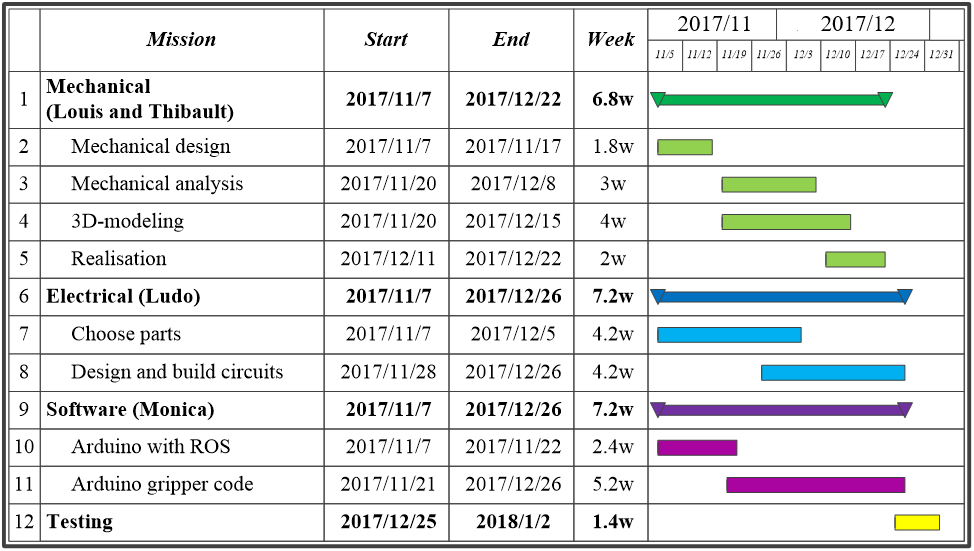
\includegraphics[width=\columnwidth]{gantt}
\centering
\caption{Gantt diagram of the project}
 \label{figure:gantt}
\end{figure}


\addtolength{\textheight}{-12cm}   % This command serves to balance the column lengths
                                  % on the last page of the document manually. It shortens
                                  % the textheight of the last page by a suitable amount.
                                  % This command does not take effect until the next page
                                  % so it should come on the page before the last. Make
                                  % sure that you do not shorten the textheight too much.

\bibliographystyle{IEEEtran}
\bibliography{egbib}

\end{document}
